% This file was created by matlab2tikz.
% Minimal pgfplots version: 1.3
%
%The latest updates can be retrieved from
%  http://www.mathworks.com/matlabcentral/fileexchange/22022-matlab2tikz
%where you can also make suggestions and rate matlab2tikz.
%
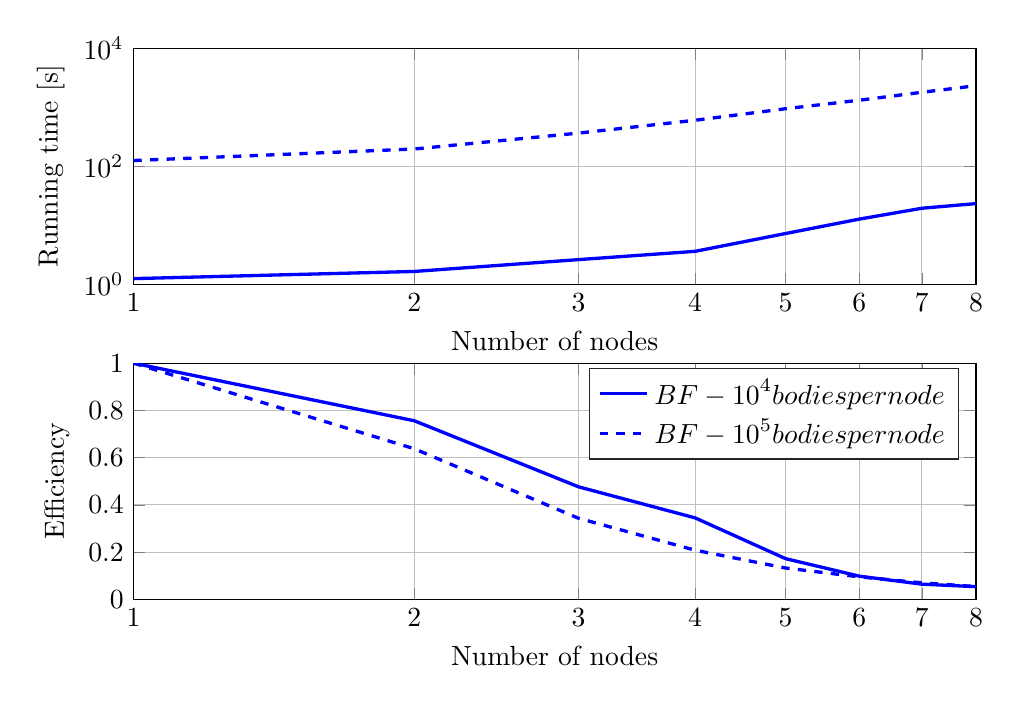
\begin{tikzpicture}

\begin{axis}[%
width=10.7cm,
height=3cm,
at={(0.758333in,1.37cm)},
scale only axis,
xmode=log,
xmin=1,
xmax=8,
xminorticks=true,
xlabel={Number of nodes},
xmajorgrids,
xminorgrids,
xtick={1, 2, 3, 4, 5, 6, 7, 8},
xticklabels={{1},{2},{3},{4},{5},{6},{7},{8}},
ymin=0,
ymax=1,
ylabel={Efficiency},
ymajorgrids,
legend style={legend cell align=left,align=left,draw=white!15!black}
]
\addplot [color=blue,solid,line width=1.2pt]
  table[row sep=crcr]{%
1	1\\
2	0.756022222489609\\
3	0.476306460007734\\
4	0.344895238110588\\
5	0.17231894047816\\
6	0.0981318273010437\\
7	0.0643015717878828\\
8	0.0536375400360533\\
};
\addlegendentry{$\text{BF - 10}^\text{4}\text{ bodies per node}$};

\addplot [color=blue,dashed,line width=1.2pt]
  table[row sep=crcr]{%
1	1\\
2	0.637555427058201\\
3	0.343172333025313\\
4	0.208015206665949\\
5	0.132620712503118\\
6	0.095214562576354\\
7	0.0699260175960599\\
8	0.0541372092748112\\
};
\addlegendentry{$\text{BF - 10}^\text{5}\text{ bodies per node}$};

\end{axis}

\begin{axis}[%
width=10.7cm,
height=3cm,
at={(0.758333in,5.37cm)},
scale only axis,
xmode=log,
xmin=1,
xmax=8,
xminorticks=true,
xlabel={Number of nodes},
xtick={1,2,3, 4, 5, 6, 7, 8},
xticklabels={{1},{2},{3},{4},{5},{6},{7},{8}},
xmajorgrids,
xminorgrids,
ymode=log,
ymin=1,
ymax=10000,
yminorticks=true,
ylabel={Running time [s]},
ymajorgrids,
yminorgrids
]
\addplot [color=blue,solid,line width=1.2pt,forget plot]
  table[row sep=crcr]{%
1	1.25145425759091\\
2	1.65531411691818\\
3	2.62741399218182\\
4	3.62850546863636\\
5	7.26243008527273\\
6	12.7527866545455\\
7	19.4622654282727\\
8	23.3316862919091\\
};
\addplot [color=blue,dashed,line width=1.2pt,forget plot]
  table[row sep=crcr]{%
1	125.071203889818\\
2	196.173067598091\\
3	364.455965279091\\
4	601.259907361818\\
5	943.07443784\\
6	1313.57221527455\\
7	1788.62186335727\\
8	2310.26322865909\\
};
\end{axis}
\end{tikzpicture}%